% gCOVguide.tex
% v4.0 released February 2015

\documentclass{gCOV2e}

\usepackage{epstopdf}% To incorporate .eps illustrations using PDFLaTeX, etc.
\usepackage{subfigure}% Support for small, `sub' figures and tables

\theoremstyle{plain}% Theorem-like structures
\newtheorem{theorem}{Theorem}[section]
\newtheorem{corollary}[theorem]{Corollary}
\newtheorem{lemma}[theorem]{Lemma}
\newtheorem{proposition}[theorem]{Proposition}

\theoremstyle{definition}
\newtheorem{definition}[theorem]{Definition}
\newtheorem{example}[theorem]{Example}

\theoremstyle{remark}
\newtheorem{remark}[theorem]{Remark}

\begin{document}

%\jvol{00} \jnum{00} \jyear{2015} \jmonth{February}

%\articletype{GUIDE}

\title{\textit{Completeness of resonance states for quantum
graph with two semi-infinite edges}}

\author{
\name{D.A. Gerasimov\textsuperscript{a}\thanks{Email:
the.dmitrii.g@gmail.com} and
I.Y.Popov\textsuperscript{a}}\thanks{$^\ast$Corresponding author.
Email: popov1955@gmail.com} \affil{\textsuperscript{a}ITMO
University, Kronverkskiy, 49, Saint Petersburg, 197101, Russia}
\received{v4.0 released February 2015} }

\maketitle

\begin{abstract}
Scattering problem for quantum graph with two semi-infinite leads
is considered. Completeness of the system of resonance states in
$L_2$ on finite subgraph is proved. A relation with the
factorization of the characteristic function in Sz-Nagy functional
model is discussed.
\end{abstract}

\begin{keywords}
scattering; resonance; completeness; functional model
\end{keywords}

\begin{classcode}     81U20; 46N50 %\textbf{(... for example; authors are encouraged to provide two to six 2010 Mathematics Subject Classification codes)}
\end{classcode}

\section{Introduction}
\subsection{Model description}

The paper is devoted to investigation of resonance states for
scattering system. The problem of resonances is intensively
studied due to its importance for physical applications (see,
e.g., \cite{ELT,APV,DEM,E,EK,Ch} and references in \cite{Pav})
There is an interesting question concerning to the completeness of
the system of such states. An example of such problem is related
to scattering by bounded obstacle
\cite{BG,HM,Gad,P90,P92,PP93,PP93a}. First, let us consider
bounded resonator $\Omega$ with smooth boundary, i.e. the Neumann
or Dirichlet Laplacian in this domain. It has the discrete
spectrum and the system of it's eigenstates is complete in
$L_2(\Omega)$. Then, consider an analogous resonator coupled with
the outer space ${\mathbb R}^3\setminus\Omega$ through a small
window. In this case the spectrum changes drastically. The
discrete spectrum disappears, in general. More precisely,
eigenvalues converge to quasi-eigenvalues (resonances) and
eigenstates - to resonance states which are similar to eigenstates
(i.e. satisfy the equation ant the boundary conditions bur do not
belong to  $L_2(\Omega\cup ({\mathbb R}^3\setminus\Omega))$).
Nevertheless, restrictions of the resonance states on $\Omega$
belong to $L_2(\Omega)$, and one can pose a question: Is the
system of the resonance states complete in $L_2(\Omega)$? At
present, there is no general answer. Our hypothesis (see
\cite{PP17}) is that the maximal appropriate domain is the convex
hull of the scatterer. In the present paper we deal with a quantum
graph (see Fig. \ref{fig:res_bundle}) having some common features
with the scattering system described above. The role of resonator
$\Omega$ is played by a number of edges connected two vertices.
Quantum graphs with included resonators were considered in a few
papers (see, e.g., \cite{BG,GEIP,EIP}). Although the number of
works concerning to resonances is very large, the problem of
resonance states completeness were considered rarely
\cite{Sh,pops,VP}. We can mention a few works in which the problem
of resonance states completeness was not declared but, really, it
was investigated (see, e.g., \cite{AIR,AI,MAAE,MM} and references
therein). As for completeness of resonance states for quantum
graph, we do not no other works dealing with this problem.


\begin{figure}[htbp]
\begin{center}
\includegraphics[trim=0 670 155 0,clip,width=\textwidth]{resonator_bundle.eps}
\caption{Quantum graph $\Gamma$, consisting of semi infinite edges
$\Omega_L, \Omega_R$ and a resonator $\Omega$, consisting of $W$
identical edges of length 1.} \label{fig:res_bundle}
\end{center}
\end{figure}

The operator $H$ on the quantum graph $\Gamma$ is defined as
follows. Schr\"{o}dinger's operator is defined on the Sobolev
space $W_2^2$ on the edges of the graph and acts as  $-\frac{d^2
\psi}{dx^2}$. At the vertices $V_a$ and $V_b$ we require the
wavefunction to be continuous. As for its derivatives, the
Kirchhoff condition takes place:

\begin{equation}\label{eq:bundle_system}
\begin{aligned}
   \forall i: \psi_i(0) &= \psi_L(0)
\\ \forall i: \psi_i(1) &= \psi_R(0)
\\ \psi'_L(0) - \sum\limits_{i = 1}^W \psi'_i(0) &= 0
\\ -\psi'_R(0) + \sum\limits_{i = 1}^W \psi'_i(1) &= 0
\end{aligned}
\end{equation}

For our purposes, it is convenient to consider the scattering in
the framework of Lax-Phillips approach \cite{Lax,Lax1}. Let us
briefly describe the approach. Consider the Cauchy problem for the
wave equation
\begin{equation}
\label{1a} \left\{
\begin{array}{ll}
u''_{tt} = H u,  \\
u(x,0)= u_0(x), u'_t(x,0)= u_1(x), x \in \Gamma.
\end{array} \right.
\end{equation}

Let $\mathcal{E}$ be the Hilbert space of two-component functions
$(u_0,u_1)$ on the graph $\Gamma$ with finite energy
$$
\| (u_0,u_1) \|_{\mathcal{E}}^2 = 2^{-1}\int_{\Gamma} (|u'_0|^2 +
|u_1|^2)dx.
$$
The pair $(u_0,u_1)$ is called the Cauchy data. Operator giving
the solution for problem (\ref{1a}), $U(t)$, $U(t) (u_0,u_1) =
(u(x,t),u'_t(x,t))$, is unitary in $\mathcal{E}$. Unitary group
$U(t)|_{t \in \mathbb{R}}$ has two orthogonal (in $\mathcal{E}$)
subspaces, $D_-$ and $D_+$, called, correspondingly, incoming and
outgoing subspaces, which are defined as follows.

\begin{definition}. Outgoing subspace $D_+$ is a subspace of
$\mathcal{E}$ having the following properties:

(a) $U(t)D_+ \subset D_+$, $t>0$;

(b) $\cap_{t>0} U(t)D_+ =\{ 0 \}$,

(c) $\overline{\cup_{t<0} U(t)D_+} = \mathcal{E}$.

 $D_-$ is defined analogously (with the natural replacement $t>0
\leftrightarrow t<0$).
\end{definition}

The following three lemmas are analogous to the corresponding
lemmas in \cite{pops}.

\begin{lemma}. Unitary group $U(t)|_{t \in \mathbb{R}}$ has a
pair of subspaces $D_{\pm}$. Particularly, one can choose
$D_{\pm}$ by the following way:
$$
D_+ = \{(u_0,u_1): -u_1=u'_0, x \in \Omega_L; u_1=u'_0, x \in
\Omega_R; u_1=u_0=0, x \in \Omega \},
$$
$$
D_- = \{(u_0,u_1): u_1=u'_0, x \in \Omega_L; -u_1=u'_0, x \in
\Omega_R; u_1=u_0=0, x \in \Omega \}.
$$
\end{lemma}
For the proof, one should directly check properties a,b,c (see
\cite{PP17}).

\begin{lemma}. There is a pair of isometric maps $T_{\pm}: \mathcal{E} \rightarrow L_2(\mathbb{R},\mathbb{C}^2)$ having the following properties:
$$
T_{\pm} U(t) = \exp{ikt} T_{\pm}, \quad T_+ D_+ =
H^2_+(\mathbb{C}^2), \quad T_- D_- = H^2_-(\mathbb{C}^2),
$$
where $H^2_{\pm}$ is the Hardy space in upper (lower) half-plane.
\end{lemma}

It is said that $T_+(T_-)$ gives one the outgoing (incoming)
spectral representation of the unitary group $U(t), U(t) =
\exp{iAt}$. Let $K= \mathcal{E}\ominus(D_+\oplus D_-).$ Consider a
semigroup $Z(t)=P_K U(t)|_K, \quad t>0$, $P_K$  is a projector to
$K$. Let $B$ be the generator of the semigroup  $Z(t): Z(t) =
\exp{iBt}, t>0$. Data which are eigenvectors of $B$ are called
resonance states \cite{Lax}. Operator $T_-T_+^{-1}$ is called the
scattering operator. It acts as a multiplication by a
matrix-function $S(k)$ which is the boundary value at the real
axis of analytic matrix-function in the upper half-plane $k$ such
that $\| S(k) \| \leq 1$ for $\Im k > 0$ and $S^* S = I$ almost
everywhere on the real axis. This analytic matrix-function $S(k)$
is called the scattering matrix.


\begin{lemma}. Map $T_-$ gives one a spectral representation for
the unitary group $U(t)$. The following relations take place.
$$
T_-D_- = H^2_-(\mathbb{C}^2), \quad T_-D_+ = S
H^2_+(\mathbb{C}^2), \quad T_- U(t) = \exp{(ikt)}T_-.
$$
Matrix-function $S$ is an inner function in $\mathbb{C}_+$ and
$$
K_- = T_- K = H^2_+\ominus S H^2_+, \quad T_- Z(t)|_K = P_{K_-}
\exp{(ikt)}T_-.
$$
\end{lemma}

As an inner function, $S$ can be  represented in the form $S = \Pi
\Theta$, where $\Pi$ is the Blaschke-Potapov product and $\Theta$
is a singular inner function \cite{Sz-N,Nik,KNP,Peller,AA}. We are
interesting in the completeness of the system of resonant states.
It is related with the factorization of the scattering matrix.

\begin{theorem}[ (Completeness criterion), \cite{Nik},
Lecture 4]\label{Nik}. Let $S$ be an inner function, $H^2_+(N)
\ominus S H^2_+(N)$, $B=P_K A \vert _K$. The following statements
are equivalent:

1. Operator $B$ is complete;

2. Operator $B^*$ is complete;

3. $S$ is a Blaschke-Potapov  product.
\end{theorem}

Here $N$ is an auxiliary space (in our case it is $\mathbb{C}^2$).

To describe the situation in more details, we will give some
preliminary remarks. We will use the following notations.

\begin{itemize}
\item $\mathbb{C}$: complex plane, $\mathbb{C} = \{ x + \mathrm{i}
y \mid x, y \in \mathbb{R} \}$
\item $\mathbb{H}$: upper complex half-plane, $\mathbb{H} =
\{ x + \mathrm{i} y \mid y > 0, x, y \in \mathbb{R} \}$
\item $\mathbb{D}$: unit disk, $\mathbb{D} = \{ z \mid
\left|z\right| < 1 \}$
\item $\mathbb{T}$: unit circle, $\mathbb{T} = \partial \mathbb{D}
=  \{z \mid \left|z\right| = 1 \}$
\item $z$ denotes a complex argument on complex plane $\mathbb{C}$
\item $\zeta$ denotes a complex argument on unit disk $\mathbb{D}$
\end{itemize}

\subsection{Cayley transform}

Cayley transform maps $\mathbb{H}$ to $\mathbb{D}$:
\[
W(z) = \frac{z - \mathrm{i}}{z + \mathrm{i}},
\]
whereas inverse Cayley transform maps $\mathbb{D}$ to
$\mathbb{H}$:
\begin{equation}\label{eq:cayley_inverse}
w(\zeta) = \mathrm{i} \frac{1 + \zeta}{1 - \zeta}.
\end{equation}

One notable property of the Cayley transform  is that it
injectively maps $\mathbb{R}$ into unit circle $\mathbb{T}$.

Another important property  we are going to use is that Cayley
transform preserves circles. In particular, a circle of radius $r,
0 < r < 1$, centered at zero, under inverse Cayley transform maps
into a circle with center at point $\mathrm{i} C(r)$ and having
the radius $R(r)$, where:

\begin{equation}\label{eq:c_and_r}
\begin{aligned}
   C(r) &= \operatorname{Im} \frac{w(r) + w(-r)}{2} =
   \frac{1 + r^2}{1 - r^2},
\\ R(r) &= \operatorname{Im} \frac{w(r) - w(-r)}{2} =
\frac{2 r}{1 - r^2}.
\end{aligned}
\end{equation}

From these formulas,  it is easy to see that if $r$ approaches
$1$, then $R(r)$ goes to infinity and $C(r)$ converges to $R(r)$.

Also, we'll note two useful facts:
\begin{subequations}
\begin{equation}
C(r) - R(r) = \frac{(1 - r)^2}{1 - r^2} > 0,
\label{eq:cr_positive}
\end{equation}
\begin{equation}
C(r) - R(r) = \frac{1 - r}{1 + r} < \frac{1}{R(r)} = \frac{1 -
r^2}{2 r} \implies C - R \text{\ is\ }
\mathcal{O}\left(\frac{1}{R}\right).
\label{eq:cr_small}
\end{equation}
\end{subequations}


\subsection{S-matrix}\label{sec:smatrix}
Our quantum graph $\Gamma$ has two semi-infinite leads
$\Omega_L,\Omega_R$. To construct the scattering matrix, we
consider two scattering problems for plane waves coming from
$\Omega_L$ and $\Omega_R$, correspondingly:
\begin{equation}\label{eq:wlwl}
\begin{aligned}
   \psi_L(x) &= A e^{\mathrm{i} k x} + B e^{-\mathrm{i} k x}
\\ \psi_R(x) &= C e^{\mathrm{i} k x} + D e^{-\mathrm{i} k x}
\end{aligned}
\end{equation}
The scattering matrix relates the final and the initial states of
the system:
\begin{equation}\label{eq:smatrix}
\begin{pmatrix} B \\ C \end{pmatrix} = S \begin{pmatrix} A \\
D \end{pmatrix},
\end{equation}
and describes scattering properties of the obstacle. In our case
the obstacle is the subgraph $\Omega$. Given $A,D$, one obtains
$B,C$ by substitution of (\ref{eq:wlwl}) into the coupling
conditions at the graph vertices (\ref{eq:bundle_system}). It
gives us the S-matrix $S(k)$.

\subsection{Completeness criterion}
There is simple criterion for absence of the singular inner factor
for the case  $\dim  N < \infty$ (for general operator case there
is no simple criterion):

\begin{theorem}[\cite{Nik}, Lecture 4 ] Let $\dim  N < \infty$. The following
statements are equivalent:

1.  $S$ is a Blaschke-Potapov  product;

2. \begin{equation}\label{eq:crit} \lim\limits_{r \to 1}
\int\limits_{C_r} \ln \left|\det S(k)\right| \frac{2
\mathrm{i}}{(k + i)^2} dk = 0,
\end{equation}
where $C_r$ is an image of $\left|\zeta\right| = r$ under the
inverse Cayley transform (\ref{eq:cayley_inverse}).
\end{theorem}

The integration curve can be parameterized as $C_r = \{R(r)
e^{\mathrm{i} t} + \mathrm{i} C(r) \mid t \in [0, 2 \pi)\}$ (see
\ref{eq:c_and_r}). For brevity, define:
\[
s(k) = \left|\det S(k)\right|,
\]
and after throwing away constants which are irrelevant for
convergence, we get the final form of the criterion, which is
convenient for us and will be used afterwards:
\begin{equation}\label{eq:critp}
\lim\limits_{r \to 1} \int\limits_{0}^{2 \pi} \ln s(R(r)
e^{\mathrm{i} t} + \mathrm{i} C(r)) \frac{R}{(R(r) e^{\mathrm{i}
t} + \mathrm{i} C(r) + i)^2} dt = 0.
\end{equation}

After solving (\ref{eq:bundle_system}) in conjunction with
(\ref{eq:wlwl}), we get the S-matrix. The expression for $S(k)$ is
rather large. We will not present it here because in the following
consideration we need only its determinant which has essentially
more simple form:
\begin{equation}\label{det-s}
\det S(k) = \frac{2 i \, W \cos\left(k\right) -
{\left(W^{2} + 1\right)} \sin\left(k\right)}{2 i \,
W \cos\left(k\right) + {\left(W^{2} + 1\right)} \sin\left(k\right)}
\end{equation}

\begin{theorem}[Main theorem] The system of resonance states for
the operator $H$ is complete in $L_2(\Omega)$.
\end{theorem}





\section{Proof of the main theorem}

Using expression (\ref{det-s}), we get:
%
\begin{equation}\label{eq:bundle_s}
s(k) = \left|\det S(k)\right| = \left|\frac{2 i \, W
\cos\left(k\right) - {\left(W^{2} + 1\right)}
\sin\left(k\right)}{2 i \, W \cos\left(k\right) + {\left(W^{2} +
1\right)} \sin\left(k\right)}\right|.
\end{equation}
%
To prove completeness, we should show that the criterion
(\ref{eq:critp}) holds for this function. We will treat the
integral as a function of $R$ and give it an upper bound such that
it vanishes as $r \to 1$ and $R \to \infty$, which means that the
integral vanishes as well, hence the completeness of resonant
states takes place.

Now, let us fix $r$, and further, for the sake of readability, we
define $C = C(r)$ and $R = R(r)$. To estimate the integral, we use
Cauchy-Schwarz's inequality:
\[
\big| \langle u,v \rangle \big| \leq \left\|u\right\|
\left\|v\right\|,
\]
or to be precise, it's $\mathcal{L}^2[a, b]$ version:
\[
\left| \int\limits_{t=a}^{b} f(t) g^*(t) dt \right| \le
\sqrt{\int\limits_{t=a}^b \left|f(t)\right|^2 dt }
\sqrt{\int\limits_{t=a}^b \left|g(t)\right|^2 dt }.
\]
%
To use the inequality, we are going to represent the integrand in
(\ref{eq:critp}) as $f(t) g^*(t)$ as follows ($a = 0, b = 2 \pi$):
\begin{equation}\label{eq:split}
f(t)   = \ln s(R e^{\mathrm{i} t} + \mathrm{i} C)
\frac{\sqrt{R}}{R e^{\mathrm{i} t} + \mathrm{i} C + i},\quad
g^*(t) = \frac{\sqrt{R}}{R e^{\mathrm{i} t} + \mathrm{i} C + i}
\end{equation}
Next, we will show that $\|g\|$ (that is, $\sqrt{\int_0^{2\pi}
\left|g(t)\right|^2}$) is bounded by a constant which does not
depend on $r$, and $\|f\|$ goes to $0$ as $r$ goes to $1$, hence
(\ref{eq:critp}) tends to zero.

\subsection{Estimating of $\|g\|$}

First, we evaluate the integrand:
\begin{align*}
\left|g(t)\right|^2 = \left|g^*(t)\right|^2 =
\frac{\sqrt{R}^2}{\left|R \cos t + \mathrm{i} R \sin t +
\mathrm{i} C + i\right|^2}
&=   \frac{R}{R^2 \cos^2 t + (R \sin t + C + 1)^2} \\
= \frac{R}{R^2 \cos^2 t + R^2 \sin^2 t + (C + 1)^2  + 2 R (C + 1)
\sin t}
&=   \frac{1}{R + \frac{(C + 1)^2}{R} + 2 (C + 1) \sin t} \\
\end{align*}
%
We integrate this function over interval $[0, 2 \pi]$. Integral of such type is well-known: % REFTODO
\[
\int\limits_{0}^{2 \pi} \frac{dx}{a_1 + a_2 \sin x} = \frac{2
\pi}{\sqrt{a_1^2 - a_2^2}},
\]
if $a_1 > a_2$. In our case, $a_1 = R + \frac{(C + 1)^2}{R}$, $a_2
= 2 (C + 1)$). First, we check that $a_1 > a_2$:
\begin{align*}
   R + \frac{(C + 1)^2}{R} - 2 (C + 1)
   &= \frac{R^2 + C^2 + 2C + 1 - 2 RC - 2 R}{R}
\\ = \frac{(C - R)^2 + 2(C - R) + 1}{R}
 &= \frac{(C - R + 1)^2 }{R}
> 0 \quad \text{,\ strictly greater since $C > R$}
\end{align*}
Next, we compute an estimate for $\sqrt{a_1^2 - a_2^2}$:
\begin{align*}
a_1^2 - a_2^2
 =  (R + \frac{(C + 1)^2}{R})^2 - (2 (C + 1))^2
& =  R^2 + \frac{(C+1)^4}{R^2} + 2 (C+1)^2 - 4 (C + 1)^2 \\
=  \left( \frac{(C + 1)^2}{R} - R \right)^2
& =  \left( \frac{(C + 1)^2 - R^2}{R}\right)^2 \\
=  \left( \frac{(C + 1 - R) (C + 1 + R)}{R}\right)^2 &\ge \left(
\frac{(1) (R + R)}{R}\right)^2  \ge 4 \quad \text{,\ since $C > R
> 0$}.
\end{align*}
Finally, since $\frac{2 \pi}{\sqrt{a_1^2 - a_2^2}} \le \frac{2
\pi}{2} = \pi$, we just proved that $\|g\|$ is bounded by a
constant.


\subsection{Estimating of $\|f\|$}
To proof the convergence, we will take into account the following
facts concerning to function $s(k)$ (\ref{eq:bundle_s}):

\begin{itemize}
\item Since $s(k)$ is an absolute value of the determinant of
the $S$ matrix, in the upper complex plane $0 \le s(k) \le 1$
holds. From here, we immediately know that the integral is bounded
from above since $ln^2 1 = 0$.
\item We replace $s(k)$ with a lower bound $l(k)$ such that:
$0 \le l(k) \le s(k) \le 1$.
\item By applying logarithm to the expression above, we get
$\ln l(k) \le \ln s(k) \le 0$, and therefore,
$\ln^2 s(k) \le \ln^2 l(k)$.
\item Now, if we prove convergence for $l(k)$, this immediately
proves the convergence of the original integral.
\end{itemize}

We are going to use this fact in our proof and do such function
changes under the integral sign, replacing complicated function
with simpler (in particular, piecewise linear) lower bounds, and
then using well known facts to estimate the integral.

\subsubsection{Simplifying of $s(k)$}

We build a simple estimate for $s(k)$ over the upper complex
plane. This function will be independent of the complex part of
its argument which will make the analysis way easier.

\begin{enumerate}
\item
  It is easy to spot that if we fix the complex part of the
  argument, $s(k)$ is periodic with respect to the real part of
  its argument.
\item
  Function $s(k)$ has countably infinite set of zeros, and each
  of them has $\operatorname{Im} k = \operatorname{arctanh}
  \frac{2 W}{W^2 + 1}$. For brevity, we define:
  \begin{equation*}
V = \frac{2 W}{W^2 + 1}, \quad Z = \operatorname{arctanh} V
  \end{equation*}
\item
  Notice that for each $x$, $s(x + \mathrm{i} y) \le
  s(\mathrm{i} y)$.
\end{enumerate}

Given these facts, we can build a simple lower bound for $s(x +
\mathrm{i} y)$:
$$
l(x + \mathrm{i} y) = \left|\frac{(W^2 + 1) \sinh y - 2 W \cosh
y}{(W^2 + 1) \sinh y + 2 W \cosh y}\right| = \left|\frac{\tanh y -
V}{\tanh y + V}\right|,
$$
since $\cosh y > 0$. It's pretty  clear that $l(k)$ has an
infinite number of zeros over the line $\operatorname{Im} k = Z$,
which implies that $\ln l(k)$ has an infinite number of
singularities over this line. Intuitively, it shouldn't spoil the
convergence of integral since the contour of integration could
intersect the singularities of the original function anyway. And
indeed, we will give a rigorous argument that we still can prove
convergence in this case. Since the function is independent from
the real part of the argument now, for brevity, we will omit it
and define $l(y) = l(\mathrm{i} y)$.

Now, we will simplify the integral  using the bound we just
constructed:
\begin{align*}
       \int\limits_{t=0}^{2 \pi} \left|f(t)\right|^2 dt
   = & \int\limits_{t = 0}^{2 \pi} \ln^2 l(R e^{\mathrm{i} t} +
   \mathrm{i} C) \frac{R}{\|R e^{\mathrm{i} t} +
   \mathrm{i} C + i\|^2} dt
\\ = & \int\limits_{t = 0}^{2 \pi} \ln^2 l(R \sin t + C)
\frac{R}{R^2 \cos^2 t + (R \sin t + C + 1)^2} dt
\end{align*}
%
First, note that:
%
\begin{equation*}
\begin{aligned}
   \sin(-\pi/2 + t)   &= \sin(-\pi/2 - t) = - \cos t,
\\ \cos^2(-\pi/2 + t) &= \cos^2(-\pi/2 = t) = \sin^2 t,
\end{aligned}
\end{equation*}
that is, the integrand is symmetric with respect to $y$ and for
proving convergence, it is enough to prove convergence on the
(half circle) contour defined by $-\pi/2 \le t \le \pi/2$.

Next, we do a variable change:
\begin{equation*}
\begin{aligned}
   y         = R \sin t + C, \quad
t      = \arcsin \frac{y - C}{R}, \quad dt        &=
\frac{1}{\sqrt{R^2 - (C - y)^2}} dy,
\\ \cos t    = \frac{\sqrt{R^2 - (C - y)^2}}{R}, \quad
y(-\pi/2) = C - R, \quad y(\pi/2)  &= C + R.
\end{aligned}
\end{equation*}
After substitution, one has:
\begin{equation}\label{eq:int_f}
\resizebox{0.9\hsize}{!}{$
\begin{aligned}
    & \int\limits_{y = C - R}^{C + R} \ln^2 l(y)
    \frac{R}{R^2 \cos^2 t + (R \sin t + C + 1)^2} dy \\
=   & \int\limits_{y = C - R}^{C + R} \ln^2 l(y)
\frac{R}{R^2 - (C - y)^2 + (y + 1)^2} \frac{1}{\sqrt{R^2 -
(C - y)^2}} dy\\
=   & \int\limits_{y = C - R}^{C + R} \ln^2 l(y)
\frac{R}{R^2 - C^2 + 2 (C + 1) y + 1} \frac{1}{\sqrt{R + C - y}}
\frac{1}{\sqrt{R - C + y}}  dy\\
\end{aligned}
$}
\end{equation}

On the integration path  we cross singularities at $y = C - R$, $y
= Z$, $y = C + R$, and the integrand is still too complex for
direct estimation. Let's split the integration path in multiple
segments and estimate them independently.

\subsubsection{Case 1: $C - R \le y \le Z$}
A crucial property of $s(k)$ is  its convergence to 1 as
$\operatorname{Im} k$ goes to 0 (which is because $s$ is the
determinant of S-matrix), since then $\ln s(k)$ goes to zero,
which is necessary to compensate the singularity of $\frac{1}{R -
C + y}$ at $y = C - R$. This means that to prove convergence using
lower bound for $s(k)$, we have to require that $s(k)$ also
converges to $1$ as $\operatorname{Im} k$ goes to $0$.

% TODO plot?
Since $l$ is convex when $0 \le y \le Z$,  we can estimate it from
below using its first derivative at $0$. However, this is not
enough, since this will violate the property of the estimate being
positive (it is under the logarithm sign), so we have to be more
careful and approximate the function at $Z$ with its first
derivative as well, and then glue them together at some point
$Z_0$:
\begin{align*}
f(y)
& =
\begin{cases}
l'(0) y + 1   &, 0 \le y < Z_0  \\
l'(Z) (y - Z) &, Z_0 \le y < Z \\
\end{cases}
\\
& =
\begin{cases}
\frac{-2}{V} y + 1   &, 0 \le y < Z_0  \\
\frac{1}{2 V}(V^2 - 1) (y - Z) &, Z_0 \le y < Z \\
\end{cases}
\end{align*}

Note that the lower bound does not have to be a continuous
function, so we can pick any number in $[C - R, Z)$ as $Z_0$. For
the ease of calculations, let's take $Z_0 = \frac{V}{4}$.

Next, we compute upper bounds for the integral \ref{eq:int_f} on
$[C - R, \frac{V}{4})$ and $[\frac{V}{4}, Z)$ separately.

%\paragraph{$C - R \le y < \frac{V}{4}$}

Note that for $C - R \le y \le \frac{V}{4}$, one has:
\begin{align*}
     A  &= \int \ln^2 l(y) \frac{R}{R^2 - C^2 + 2 (C + 1) y + 1}
       \frac{1}{\sqrt{R + C - y}} \frac{1}{\sqrt{R - C + y}}dy
\\ \le & \int \ln^2 (1 - \frac{2}{V} y) \frac{R}{R^2 - C^2 +
2 (C + 1) y + 1} \frac{1}{\sqrt{R + C - Z}} \frac{1}{\sqrt{R - C +
y}}dy
\end{align*}

Now, we use a well known inequality which holds for $x > -1$:
\[
\frac{x}{1 + x} \le \ln (1 + x),
\]
where in our case $x = -\frac{2}{V} y$. Since the expression under
logarithm is less than 1, we get $\ln^2 (1 + x) \le \frac{x^2}{(1
+ x)^2}$:
\begin{align*}
       A \le & \int \frac{\frac{4}{V^2}y^2}{(1 - \frac{2}{V}y)^2}
       \frac{R}{R^2 - C^2 + 2 (C + 1) y + 1} \frac{1}{\sqrt{R +
       C - Z}} \frac{1}{\sqrt{R - C + y}}dy
\\ \le & \int \frac{\frac{4}{V^2}y^2}{(1 - \frac{2}{V}
\frac{V}{4})^2}  \frac{R}{R^2 - C^2 + 2 (C + 1) y + 1}
\frac{1}{\sqrt{R + C - Z}} \frac{1}{\sqrt{R - C + y}}dy
\\ =   & \frac{\frac{4}{V^2}}{(1 - \frac{2}{V} \frac{V}{4})^2}
\frac{R}{\sqrt{R + C - Z}}  \int \frac{y^2}{R^2 - C^2 + 2 (C + 1)
y + 1}  \frac{1}{\sqrt{R - C + y}}dy
\end{align*}

It's clear that the multiplier before the integral has order
$\mathcal{O}(\sqrt{R})$ (we can ignore the terms dependent on
$V$ only since $V$ is a constant independent of $r$).

The first part of the integrand has the form $\frac{y^2}{a + b
y}$, where $a = R^2 - C^2 + 1, b = 2 (C + 1)$; when $R$ and $C$
are large enough, $a > 0$ and $b > 0$. That means $\frac{y^2}{a +
b y}$ will be non-negative when $y > 0$, and non decreasing,
since:
\[
  \left(\frac{y^2}{a + b y}\right)'
= \frac{2y}{a + by} + y^2 \frac{-b}{(a + by)^2} = \frac{2y (a +
by) - b y^2}{(a + by)^2} = \frac{y (2a + by)}{(a + by)^2} \ge 0.
\]
This implies that we can estimate the function from above by using
its value on the rightmost point of the interval at $\frac{V}{4}$.
\[
\frac{y^2}{a + b y} \le \frac{\frac{V^2}{16}}{R^2 - C^2 + 1 + 2 (C
+ 1) \frac{V}{4}} = \mathcal{O}\left(\frac{1}{R}\right).
\]

Integral of the second part of the integrand is:
$$
\int\limits_{C - R}^{\frac{V}{4}} \frac{1}{\sqrt{R - C + y}}dy
    = 2 \sqrt{\frac{V}{4} - (C - R)}
< 2 \sqrt{\frac{V}{4}}  = \mathcal{O}(1),
$$
since $C - R > 0$, see (\ref{eq:cr_positive}). Finally, after
combining, we get $\mathcal{O}(\sqrt{R})
\mathcal{O}\left(\frac{1}{R}\right) \mathcal{O}(1)  =
\mathcal{O}\left(\frac{1}{\sqrt{R}}\right)$.

%\paragraph{$\frac{V}{4} \le y < Z$}

Note that for $\frac{V}{4} \le y < Z$:
\begin{align*}
       & \int \ln^2 l(y) \frac{R}{R^2 - C^2 + 2 (C + 1) y + 1}
       \frac{1}{\sqrt{R + C - y}} \frac{1}{\sqrt{R - C + y}}dy
\\ \le & \int \ln^2 l(y) \frac{R}{R^2 - C^2 + 2 (C + 1) \frac{V}{4}
+ 1} \frac{1}{\sqrt{R + C - Z}} \frac{1}{\sqrt{R - C +
\frac{V}{4}}}dy
\\ \le &  \frac{R}{R^2 - C^2 + 2 (C + 1) \frac{V}{4} + 1}
\frac{1}{\sqrt{R + C - Z}} \frac{1}{\sqrt{R - C + \frac{V}{4}}}
\int \ln^2 \left( \frac{1}{2 V}(V^2 - 1) (y - Z) \right)dy.
\end{align*}

First, take a look  at the multiplier before the integral, using
(\ref{eq:cr_small}) it is pretty clear, it has order of growth
$\mathcal{O}\left(\frac{1}{\sqrt{R}}\right)$.

As for the integral, $\ln^2(x)$ is integrable in the neighborhood
of $x = 0$, and it is known that:
\[
\int\limits_{x=x_0}^b \ln^2(a (x - b)) dx = (b - x_0) (\ln^2(a
(x_0 - b)) - 2 \ln(a (x_0 - b)) + 2).
\]
In our case $x_0 = \frac{V}{4}$, $a = \frac{1}{2 V}(V^2 - 1)$, $b
= Z$, and we can see that the integral is bounded by a constant
independent of $R$ and $C$, hence, the integral on this interval
grows as $\mathcal{O}(\frac{1}{\sqrt{R}})$.

\subsubsection{Case 2: $y > Z$}
If $y > Z$ then
\[
l(x + \mathrm{i} y)
 = \frac{\tanh y - V}{\tanh y + V}
 = 1 - 2 \frac{V}{\tanh y + V}
\]
Since $l$ is concave, strictly increasing and for a fixed $r$, we
are only interested at $y \le C + R$, we can estimate the function
by a linear one:
\[
f(y) = \frac{l(C + R)}{C + R - Z} (y - Z)
\]
Note that when $y = C + R$, for a sufficiently big $r$, $l(y)$ is
bounded from both sides by constants, independent from $C$ and
$R$. This is because $\tanh y$ goes to $1$ as $y$ goes to
infinity, therefore, $l(y)$ in the limit will be equal to $1 -
\frac{2 V}{V + 1}$. This is an important property of this specific
model, since if $l$ went to zero at infinity, this part of the
proof couldn't have been done.

First, note that for $Z \le y \le R + C$ the function
$\frac{1}{\sqrt{R - C + y}}$ has no singularities, and we can
estimate the integral (\ref{eq:int_f}) as:
\begin{equation}\label{eq:int_f_up}
\begin{aligned}
       & \int \ln^2 l(y) \frac{R}{R^2 - C^2 + 2 (C + 1) y + 1}
       \frac{1}{\sqrt{R + C - y}} \frac{1}{\sqrt{R - C + y}}dy
\\ \le & \int \ln^2 l(y) \frac{R}{R^2 - C^2 + 2 (C + 1) y + 1}
\frac{1}{\sqrt{R + C - y}} \frac{1}{\sqrt{R - C + Z}}dy
\end{aligned}
\end{equation}

To estimate  this expression, let's split the integration path in
three intervals: $[Z, Z + \frac{1}{R})$, $[Z + \frac{1}{R}, C)$,
$[C, C + R]$.
%
%\paragraph{$Z \le y < Z + \frac{1}{R}$}

Consider the case $Z \le y < Z + \frac{1}{R}$.
%
Let's estimate (\ref{eq:int_f_up}), replacing functions  under the
integral sign by their extreme value at interval's ends:
\begin{align*}
       & \int \ln^2 l(y) \frac{R}{R^2 - C^2 + 2 (C + 1) y + 1}
       \frac{1}{\sqrt{R + C - y}} \frac{1}{\sqrt{R - C + Z}}dy
\\ \le & \int \ln^2 l(y) \frac{R}{R^2 - C^2 + 2 (C + 1) Z + 1}
\frac{1}{\sqrt{R + C - (Z + \frac{1}{R})}} \frac{1}{\sqrt{R - C +
Z}}dy
\\ =   & \frac{1}{\sqrt{R + C - (Z + \frac{1}{R})}}
\frac{1}{\sqrt{R - C + Z}} \frac{R}{R^2 - C^2 + 2 (C + 1) Z + 1}
\int \ln^2 l(y)dy.
\end{align*}

Using (\ref{eq:cr_small}), it is easy to see  that the coefficient
before the integral has order of growth
$\mathcal{O}\left(\frac{1}{\sqrt{R}}\right)$.

As for the integral $\int\limits_{Z}^{Z + \frac{1}{R}} \ln^2 l(y)
dy$, it can be computed explicitly, using:
\[
    \int\limits_b^{b + c} \ln^2 (a (x - b)) dx = c (\ln^2(a c) - 2 \ln (a c) + 2)
\]
Hence,
$$
\int\limits_{Z}^{Z + \frac{1}{R}} \ln^2 l(y) dy = \frac{1}{R} (
\ln^2 (\frac{l(C + R)}{C + R - Z} \frac{1}{R}) - 2 \ln (\frac{l(C
+ R)}{C + R - Z} \frac{1}{R}) + 2).
$$
As we noted
above, $l(C + R)$ is bounded by positive constants less than $1$
and independent of $r$, and we can see that the expression grows
as $\mathcal{O}(\frac{\ln^2 R}{R})$.

By combining the estimates for the coefficient and the integral,
we get $\mathcal{O}(\frac{\ln^2 R}{R \sqrt{R}})$.

%\paragraph{$Z + \frac{1}{R} \le y < C$}
The next case is $Z + \frac{1}{R} \le y < C$.

Again, by picking extreme  values for the parts of integrands, we
can estimate (\ref{eq:int_f_up}) as:
\begin{align*}
       & \int \ln^2 l(y) \frac{R}{R^2 - C^2 + 2 (C + 1) y + 1}
       \frac{1}{\sqrt{R + C - y}} \frac{1}{\sqrt{R - C + Z}}dy
\\ \le & \int \ln^2 l(Z + \frac{1}{R}) \frac{R}{R^2 - C^2 +
2 (C + 1) y + 1} \frac{1}{\sqrt{R + C - C}} \frac{1}{\sqrt{R - C +
Z}}dy
\\  =  & \ln^2 l(Z + \frac{1}{R})  \frac{R}{\sqrt{R + C - C}}
\frac{1}{\sqrt{R - C + Z}} \int \frac{1}{R^2 - C^2 + 2 (C + 1) y +
1}dy
\end{align*}
As $R$ goes to infinity, $\ln^2 l(Z + \frac{1}{R})$ goes to
infinity as well, so we have to compute the order of singularity.
Since $\ln l(Z + \frac{1}{R}) = \ln \left( \frac{l(C + R)}{C + R -
Z} \frac{1}{R} \right) = \ln l(C + R) - \ln (C + R - Z) - \ln R$,
we can see that $\ln^2 l(Z + \frac{1}{R}) = \mathcal{O} (\ln^2
R)$.


As for the integral, it is well known that:
\[
\int \frac{1}{a x + b}dx = \frac{\ln (a x + b)}{a} +c.
\]
In our case $a = 2 (C + 1)$, $b = R^2 - C^2 + 1$. Substituting the
ends of the interval $(Z + \frac{1}{R}, C)$, we get the value of
our integral over interval $(Z + \frac{1}{R}, C)$:
\[
\frac{\ln \frac{2 (C + 1) C + R^2 - C^2 + 1}{2 (C + 1) (Z +
\frac{1}{R}) + R^2 - C^2 + 1}}{2 (C + 1)} = \mathcal{O}\left(
\frac{\ln R}{R} \right).
\]


Finally, after combining, we  get:
$$
\mathcal{O} (\ln^2 R) \frac{R}{\sqrt{R}} \frac{1}{\sqrt{R - C +
Z}} \mathcal{O}\left( \frac{\ln R}{R} \right)  = \mathcal{O}\left(
\frac{\ln^3 R}{\sqrt{R}} \right).
$$

%\paragraph{$C \le y \le C + R$}
The last case is $C \le y \le C + R$.

Again, estimating (\ref{eq:int_f_up}) from above, one obtains:
\begin{align*}
       & \int \ln^2 l(y) \frac{R}{R^2 - C^2 + 2 (C + 1) y + 1}
       \frac{1}{\sqrt{R + C - y}} \frac{1}{\sqrt{R - C + Z}}dy
\\ \le & \int \ln^2 l(C) \frac{R}{R^2 - C^2 + 2 (C + 1) C + 1}
\frac{1}{\sqrt{R + C - y}} \frac{1}{\sqrt{R - C + Z}}dy
\\ =   & \ln^2 l(C) \frac{R}{R^2 - C^2 + 2 (C + 1) C + 1}
\frac{1}{\sqrt{R - C + Z}} \int \frac{1}{\sqrt{R + C - y}}dy
\end{align*}

Integral of $\frac{1}{\sqrt{R + C - y}}$ from $C$ to $C + R$ is
elementary and equals $2 \sqrt{R}$. Function $f$ at $C$ is bounded
by constants not dependent on $r$, therefore, the square of its
logarithm is bounded as well. Finally, we get an expression of
order $\mathcal{O} \left( \frac{1}{R} \right) \mathcal{O}( \sqrt R
) = \mathcal{O} \left( \frac{1}{\sqrt{R}} \right)$.

\subsubsection{Final estimate of $\int_0^{2\pi} \left|f(t)\right|^2 dt$}
We have split our integration path in five intervals, and the
integral has the order:
\[
\mathcal{O} \left( \frac{1}{\sqrt{R}} \right) + \mathcal{O} \left(
\frac{1}{\sqrt{R}} \right) + \mathcal{O}\left(\frac{\ln^2 R}{R
\sqrt{R}}\right) + \mathcal{O}\left( \frac{\ln^3 R}{\sqrt{R}}
\right) + \mathcal{O} \left( \frac{1}{\sqrt{R}} \right) =
\mathcal{O}\left( \frac{\ln^3 R}{\sqrt{R}} \right),
\]
which means that the integral converges to $0$ as $r$ goes to $1$
and $R$ goes to $\infty$. Correspondingly, the proof of the main
theorem is complete.


\section*{Acknowledgements}

This work was partially financially supported by  the Government
of the Russian Federation (grant 074-U01), by grant MK-5161.2016.1
of the President of the Russian Federation, DFG Grant NE~1439/3-1,
by grant 16-11-10330 of Russian Science Foundation.

\begin{thebibliography}{99}

\bibitem{ELT} P. Exner, V. Lotoreichik, M. Tater On resonances and bound
states of Smilansky Hamiltonian. Nanosystems: Phys. Chem. Math.
{\bf 7} (2016), 789-802.

\bibitem{APV} A.Aslanyan, L.Parnovski and D.Vassiliev. Complex resonances
in acoustic waveguides. Q. J. Mech. Appl. Math. 53 (3) (2000),
429-447.

\bibitem{DEM} P.Duclos, P.Exner, B.Meller. Open quantum dots: Resonances
from perturbed symmetry and bound states in strong magnetic
fields. Rep. Math. Phys. 47 (2) (2001), 253-267.

\bibitem{E} J.Edward. On the resonances of the Laplacian on waveguides. J.
Math. Anal. Appl. 272 (1) (2002), 89-116.


\bibitem{EK} P.Exner, H.Kovarik. Quantum waveguides. Springer, Ber;in (2015).

\bibitem{Ch} T.Christiansen. Some upper bounds on the number of resonances
for manifolds with infinite cylindrical ends. Ann. Henri Poincare,
3 (2002), 895--920.

\bibitem{Pav} I.Y.Popov, P.A. Kurasov, S.N. Naboko, A.A. Kiselev,
A.E. Ryzhkov, A.M. Yafyasov, G.P. Miroshnichenko, Yu.E.
Karpeshina, V.I. Kruglov, T.F. Pankratova, A.I. Popov. A
distinguished mathematical physicist Boris S. Pavlov. Nanosystems:
Phys. Chem. Math. {\bf 7} (2016), 782--788.

\bibitem{HM}
 P.D.Hislop,  A.Martinez, Scattering  resonances of Helmholtz
resonator, Indiana Univ. Math. J. 40 (1991), 767--788.

\bibitem{Gad}
R.R.Gadyl'shin,  Existence and asymptotics  of poles with small
imaginary part for the Helmholtz resonator, Russian Mathematical
Surveys, 52 (1) (1997), 1--72.

\bibitem{P90}
I.Y.Popov,  Extension theory and localization of resonances for
domains of trap type,  Mathematics of the USSR-Sbornik, 71 (1)
(1992), 209--234. DOI: 10.1070/SM1992v071n01ABEH001394

\bibitem{P92}
 I.Y.Popov, The resonator with narrow slit and the model based on
the operator extensions theory, J. Math. Phys., 33 (11) (1992),
3794--3801.

\bibitem{PP93}
I.Y.Popov, S.L. Popova,  Zero-width slit model and resonances in
mesoscopic systems, Europhysics Letters, 24 (5) (1993), 373--377.

\bibitem{PP93a}
I.Y.Popov, S.L. Popova,  The extension theory and resonances for a
quantum waveguide, Physics Lett. A. 173 (1993), 484-- 488.

\bibitem{BG} J.~Bruning, V.~A.~Geyler, Scattering on compact manifold
with infinitely thin horns, J. Math. Phys. 44 (2003), 371--405.

\bibitem{PP17} I.Y.Popov, A.I.Popov. Line with attached segment as a model of
Helmholtz resonator: Resonant states completeness. Journal of King
Saud University � Science. {\bf 29} (2017), 133--136.

\bibitem{GEIP} E. N. Grishanov, D. A. Eremin, D. A. Ivanov,
and I. Yu. Popov. Dirac operator on the sphere with attached
wires. Chin. Phys. B  {\bf 25} (4) (2016), 047303/1-4.

\bibitem{EIP} D.A.Eremin,  D.A.Ivanov, I.Y.Popov. Model of
tunnelling through nanosphere in a magnetic field. Physica E, {\bf
44} (2012), 1598-1601.

\bibitem{Sh}
A.A.Shushkov.  Structure of resonances for symmetric scatterers.
Theor. Math. Phys. {\bf 64} (1985), 944 -- 949.

\bibitem{pops} I.Yu. Popov, A.V. Strepetov. On the completeness
of eigenfunctions for bilateral Regge problem. Leningrad Univ.
Vestnik. Mathematics. No 13 (1983), 25--31.

\bibitem{VP}
A.M.Vorobiev, I. Y.Popov,  2015.  Model of quantum dot and
resonant states for the Helmholtz resonator. J. Phys.: Conf.
Series. {\bf 643} (2015), 012097.

\bibitem{AIR} S. A. Avdonin, S. A. Ivanov, D. L. Russell,
Exponential bases in Sobolev spaces in control and observation
problems for the wave equation. Proc. Roy. Soc. Edinburgh Sect. A
{\bf 130} (2000), 947�-970.

\bibitem{AI} S. Avdonin, S. A. Ivanov. {\it Families of exponentials.
The method of moments in controllability problems for distributed
parameter systems}. Cambridge Univ. Press, Cambridge, 1995.

\bibitem{MAAE} F. Al-Musallam, S. Avdonin, N. Avdonina, J.
Edward. Control and inverse problems for networks of vibrating
strings with attached masses. Nanosystems: Phys. Chem. Math. {\bf
7} (2016), 835--841.

\bibitem{MM} A. S. Mikhaylov, V. S. Mikhaylov. Dynamical inverse
problem for the discrete Schr\"{o}dinger operator. Nanosystems:
Phys. Chem. Math. {\bf 7} (2016), 842--853.

\bibitem{Lax} P.D.Lax  and R.S.Phillips.  {\it Scattering theory}.
Academic Press, New York (1967)

\bibitem{Lax1} P.D.Lax  and R.S.Phillips.  {\it Scattering theory for
automorphic functions}. Princeton Univ. Press, Princeton, N. J.,
and Univ. of Tokyo Press, Tokyo (1976).

\bibitem{Sz-N} B.Sz.-Nagy, C.Foias, H.Bercovici, L.Kerchy.
{\it Harmonic Analysis of Operators on Hilbert Space}, 2nd
edition. Springer, Berlin (2010).

\bibitem{Nik}
N.Nikol'skii. {\it Treatise on the shift operator: spectral
function theory}. Springer Science \& Business Media; Berlin,
(2012).

\bibitem{KNP} S. V.Khrushchev, N.K.Nikol'skii, B.S.Pavlov.
Unconditional bases of exponentials and of reproducing kernels,
Complex Analysis and Spectral Theory (Leningrad, 1979/1980),
Lecture Notes in Math., vol. 864, Springer-Verlag, Berlin�New
York, 214�-335 (1981).

\bibitem{Peller} V. V.Peller. {\it Hankel Operators and Their Applications.
 Springer Monographs in Mathematics}. Springer-Verlag, New York (2003).

\bibitem{AA}  V.M.Adamyan ,  D.Z.Arov. On a class of scattering operators
and characteristic operator-functions of contractions. Dokl. Akad.
Nauk SSSR, {\bf 160} (1965), 9-12.



\end{thebibliography}
\end{document}
